\begin{appendices}
\pagecolor{LightSteelBlue1}
\chapter{Appendix A}
\label{appendix_a}

\section{Reinforcement Learning approach} As noted in the preceding section the process of solving a subproblem after selecting a variable to add to the partial solution resembles the procedure followed when training models in a reinforcement learning type setting. Creating the labeled training and testing datasets is an expensive operation. Even when using state of the art heuristics for extracting high quality solution for large problems the process can easily take days. As a consequence of this it cannot be argued that these methods scale properly to larger instances. Unsupervised methods of training our models could provide an attractive alternative but require modification of the predicted quantities an loss function. 

\begin{figure}[h]
	\centering
	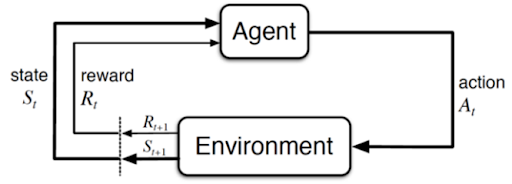
\includegraphics[width=.5\textwidth]{resources/img/markov_decision_process.png}
	\caption{Markov decision process: an iterative process in which an agent interacts with an environment (represented by its state at iteration $t$ $S_t$). The environment provides the agent with a set of possible actions $\{A_t^1, ..., A_t^{\alpha}\}$, the agent selects an action $A_t$, is rewarded with $R_t$ and the environment state is updated. The agents objective is to maximize its total reward $\sum_t R_t$.}
	\label{fig:mdp}
\end{figure}

In a Q-learning setting the target of the model is to predict the discounted reward obtained at the end of an "episode" if action $a_t$ is taken at iteration $t$. The objective we are trying to minimize is the difference between the predicted discounted reward $\gamma_{\theta}(a_t | P_t)$ and the incured reward plus the best discounted predicted reward in state $t+1$: $r_{a_t} + \lambda \max_{a\in A_{t+1}} \gamma_{\theta}(a | P_{t+1})$ .

In the MIS setting we can define:
\begin{itemize}
	\item State $S_t$: bipartite/factor-graph representation of the problem at current iteration (restriction to graph induced by remaining candidate vertices $W_t$)
	\item Actions are $W_t$
	\item All actions result is a reward $R_t = 1$
	\item Current implementations of our Nair+MRF models use the Sum-Product algorithm for producing estimated marginals $\mu_F(x_F)$. Replacing the Sum-Product by Max-Sum the estimations become max-pseudo-marginals $\Phi_F(x_F) = \max_{x': x'=x_F} E(x)$. We have shown that their exists an sequence of MRFs converging to with $E(x) \propto c(x)$ for $x\in\mathcal{F}$ and $E(x) = 0$ for $x\notin \mathcal{F}$. 
\end{itemize}


\section{Wasserstein distance unsupervised} Reinforcement learning can suffer from unstable learning, especially with sparse rewards. Although the MIS problem seems particularly well suited for this framework it might not be the case for other problems. In this section we present an outline of an unsupervised training method based on ranking and using the Wasserstein distance. Given a CO problem $P$ with cost function $c(x)$ with finite value on the feasible set $\mathcal{F}$ and $c(x)=\infty$ if $x\notin \mathcal{F}$ and a set of solutions $\{ x_i \}_{i\in\mathbb{N}}$, the idea is to train a MRF based model to imitate the ordering defined by $c(x)$. 

Assume that the target distribution is $p^*(x) \propto \exp c(x)$ and the model we want to fit is $p_{\theta}(x) \propto \exp \langle \theta , \phi(x) \rangle$. 


\newpage
\pagecolor{Wheat1}
\chapter{Appendix B}
\label{appendix_b}

\section{Clique cover construction.}  
Finding all maximal cliques is itself hard, but approximate coverings can be obtained efficiently. Algorithm~\ref{alg:clique_cover} sketches a simple constructive procedure for generating a clique cover.

\begin{algorithm}[H]
\caption{Covering a graph with maximal cliques}\label{alg:clique_cover}
\KwData{$G = (V,E)$}
\KwResult{Set of cliques $\mathcal{C} = \{ c : c\subseteq V \}$}
$\mathcal{C} = \emptyset$\;
$m(u,v) = 0 \quad \forall (u,v) \in E$\;
\While{$E \neq \emptyset$}{
  $c \gets$ select edge $(u,v)$ with $m(u,v)=0$\;
  $W = N(u) \cap N(v)$\;
  \While{$ W \neq \emptyset$}{
      $w \gets$ select in $W$\;
      $C \gets C \cup \{ w \}$\;
      $W = W \cap N(w)$\;
      $m(w,u) = 1 \quad \forall u \in C$\;
  }
  $\mathcal{C} \gets \mathcal{C} \cup \{ C \}$\;
}
\end{algorithm}


\end{appendices}

\newpage
\pagecolor{lightmauve}
\chapter{Appendix C}
\label{appendix_c}

\section{Inferring MIS solutions without training, alternate sampling methods and results}

This appendix complements the main results by examining two ablation variants in which we \emph{do not train} the MRF parameters. Instead, factor potentials are set deterministically from feasibility information and then used with fixed-iteration message passing to produce beliefs, which are decoded either greedily or via importance sampling (IS). These experiments isolate the value of learned potentials by asking: how far can one go with handcrafted feasibility-driven potentials on loopy factor graphs?

\paragraph{Common setting.}
We use the same MIS instance families and graph encodings as in the main text. For each partial assignment (during decoding), we update potentials according to the rules described below and then run sum–product (SP) or max–sum (MS) belief propagation for a fixed number of iterations with light damping; on loopy graphs, convergence is \emph{not} guaranteed and we report the last iterate. Decoding uses either a greedy policy guided by unary beliefs or IS with the beliefs serving as proposal/weights, consistent with the main experimental protocol.

\subsection{Variant A: Soft Feasibility Penalty (Nonzero Potentials)}
\label{app:soft_penalty}
\textbf{Definition.}
Let $x_\alpha$ be a local assignment for factor $\alpha$ (e.g., a clique or constraint scope). Define a simple violation indicator $v_\alpha(x_\alpha)\in\{0,1\}$ that is $1$ if $x_\alpha$ conflicts with the current partial solution or violates the local combinatorial constraint, and $0$ otherwise. We assign
\[
\psi_\alpha(x_\alpha) \;=\; 
\begin{cases}
\eta_{\text{feas}} & \text{if } v_\alpha(x_\alpha)=0,\\[2pt]
\eta_{\text{inf}}  & \text{if } v_\alpha(x_\alpha)=1,
\end{cases}
\qquad \text{with } \; 0<\eta_{\text{inf}}<\eta_{\text{feas}}.
\]
All assignments remain \emph{strictly} positive, but infeasible ones are down-weighted. In practice we use a fixed ratio $\eta_{\text{feas}}/\eta_{\text{inf}}>1$ to maintain numerical stability while biasing beliefs toward feasibility.

\textbf{Rationale.}
This “soft mask’’ encourages feasibility without collapsing potentials to zero, which can stall message passing or create brittle dynamics when many factors simultaneously rule out large portions of the local state space.

\textbf{Results and interpretation.}
Table~\ref{tab:soft_penalty_results} (Appendix) reports gaps for SP/MS with greedy and IS decoders. Trends are consistent across formulations: SP+IS improves upon SP+greedy, but both remain \emph{substantially} worse than trained models; MS is generally less stable and inferior here. Overall, keeping all assignments marginally viable does not compensate for the lack of learned, instance-adapted potentials; feasibility structure alone is too weak to drive high-quality solutions on loopy graphs.

\subsection{Variant B: Unary-Only Updates (Higher-Order Potentials Frozen)}
\label{app:unary_only}
\textbf{Definition.}
When a partial assignment fixes a subset of variables, we only modify \emph{unary} factors to reflect those fixed values (and optionally light preferences for unfixed variables), while \emph{keeping all higher-order factors unchanged}. This preserves computational simplicity and avoids repeatedly reconfiguring large factor tables during decoding.

\textbf{Rationale.}
This variant tests whether inexpensive potential updates can suffice when the factor graph is complex. It is attractive computationally, but it abandons the opportunity to re-encode evolving feasibility at the constraint level.

\textbf{Results and interpretation.}
Table~\ref{tab:unary_only_results} (Appendix) summarizes performance by formulation category. Unary-only updates yield the lowest overhead but also the weakest guidance: gaps remain high for both SP and MS; SP+IS is consistently better than SP+greedy yet still far from trained MRFs. Freezing higher-order factors deprives inference of the very constraint coupling it needs to steer decoding away from combinatorial conflicts.

\subsection{Discussion and Takeaways}
Across both ablations, we observe:
\begin{itemize}
  \item \textbf{No convergence guarantees.} On the loopy factor graphs considered, SP/MS often fail to converge; using a fixed number of iterations with damping mitigates but does not eliminate poor fixed points.
  \item \textbf{IS helps but is not sufficient.} Importance sampling on top of these untrained beliefs reliably improves gaps over greedy, yet it cannot close the gap to the learned models.
  \item \textbf{Learned structure is key.} Handcrafted feasibility signals—whether softly penalized or restricted to unaries—do not substitute for learned potentials that encode instance-specific structure. This reinforces the central claim of the paper: \emph{amortized, differentiable inference over a GNN-parameterized MRF materially improves solution quality}.
\end{itemize}

For numerical details, see Table~\ref{tab:soft_penalty_results} (soft feasibility penalty) and Table~\ref{tab:unary_only_results} (unary-only updates). Together with the main text, these ablations clarify that feasibility-only heuristics produce fragile beliefs and inferior solutions, whereas learning the MRF parameters—and running even a modest number of BP iterations—substantially boosts performance.


\begin{table}[!ht]
    \centering
    \begin{tabular}{l|r|r|r|r}
    \hline
        \textbf{Formulation} & \textbf{SP+Greedy} & \textbf{SP+IS} & \textbf{MS+Greedy} & \textbf{MS+IS} \\ \hline
        MIS100\_EB & $13.737 (\pm 4.925)$ & $\mathbf{6.478 (\pm 4.321)}$ & $37.001 (\pm 6.369)$ & $30.769 (\pm 6.411)$ \\
        MIS100\_CC & $14.186 (\pm 5.255)$ & $\mathbf{9.947 (\pm 4.827)}$ & $33.050 (\pm 7.347)$ & $28.603 (\pm 6.688)$ \\
        MIS100\_CF & $13.737 (\pm 4.925)$ & $\mathbf{6.478 (\pm 4.321)}$ & $37.001 (\pm 6.369)$ & $30.769 (\pm 6.411)$ \\
        MIS100\_EC & $13.971 (\pm 4.901)$ & $\mathbf{11.515 (\pm 4.679)}$ & $35.155 (\pm 6.708)$ & $30.112 (\pm 7.054)$ \\
        MIS100\_CP & $13.889 (\pm 5.456)$ & $\mathbf{9.872 (\pm 5.025)}$ & $33.454 (\pm 6.849)$ & $28.513 (\pm 6.556)$ \\ \hline
    \end{tabular}
    \caption{Optimality gap comparison for Sum-Product and Max-Sum belief propagation algorithm inference, with greedy and importance sampling (V2: only unary factor parameters are changed) solvers. The model is defined following the "idealized" models such as defined in \ref{equ:idealized_mrf} but parameters are set to values $\theta_{r:x_r}=1$ if $A_r^T x_r \leq b_r$ and $\theta_{r:x_r}=0$ otherwise.}
    \label{tab:soft_penalty_results}
\end{table}

\begin{table}[!ht]
    \centering
    \begin{tabular}{l||r|r|r|r}
    \hline
        \textbf{Cat} & \textbf{SP+Greedy} & \textbf{SP+IS} & \textbf{MS+Greedy} & \textbf{MS+IS} \\ \hline
        EB & $14.072 (\pm 4.576)$ & $\mathbf{4.500 (\pm 3.800)}$ & $13.220 (\pm 3.590)$ & $23.142 (\pm 7.354)$ \\
        CC & $11.518 (\pm 4.752)$ & $\mathbf{4.917 (\pm 4.761)}$ & $14.472 (\pm 3.856)$ & $25.174 (\pm 8.768)$ \\
        CF & $14.072 (\pm 4.576)$ & $\mathbf{4.500 (\pm 3.800)}$  & $13.220 (\pm 3.590)$ & $23.142 (\pm 7.354)$ \\
        EC & $21.056 (\pm 4.846)$ & $\mathbf{11.535 (\pm 4.726)}$ & $12.370 (\pm 4.449)$ & $25.991 (\pm 8.489)$ \\
        CP & $13.656 (\pm 4.238)$ & $\mathbf{5.351 (\pm 4.483)}$ & $13.222 (\pm 4.842)$ & $24.391 (\pm 9.750)$ \\ \hline
    \end{tabular}
    \caption{Optimality gap comparison for Sum-Product and Max-Sum belief propagation algorithm inference, with greedy and importance sampling (V2: only unary factor parameters are changed) solvers. The model is defined following the "idealized" models such as defined in \ref{equ:idealized_mrf}}
    \label{tab:unary_only_results}
\end{table}

\newpage
\pagecolor{lightmauve}
\chapter{Appendix D}
\label{appendix_d}

% equations before the algorithm
\begin{align}
r_{F \to Y_i}(y_i) &= \log \sum_{\substack{y'_F \in Y_F \\ y'_i = y_i}}
   \exp\!\left(-E_F(y'_F) + \sum_{j \in N(F)\setminus\{i\}} q_{Y_j \to F}(y'_j)\right), \label{eq:lbf_fac2var}\\
\bar q_{Y_i \to F}(y_i) &= \sum_{F' \in M(i)\setminus\{F\}} r_{F' \to Y_i}(y_i), \label{eq:lbf_var2fac_raw}\\
q_{Y_i \to F}(y_i) &= \bar q_{Y_i \to F}(y_i) -
   \log \sum_{y_i \in Y_i}\exp\!\big(\bar q_{Y_i \to F}(y_i)\big). \label{eq:lbf_var2fac}
\end{align}

% algorithm
\begin{algorithm}[H]
\caption{Loopy Belief Propagation (Sum–Product)}
\KwIn{$(V,F,E)$, energies $E_F$, tolerance $\varepsilon$, max iters $T$}
\KwOut{Beliefs $\mu_i$, $\mu_F$, approx.\ $\log Z$}
\BlankLine
Initialize $q_{Y_i\to F}(y_i)\gets 0$ for all edges and states\;
\For{$t=1$ \KwTo $T$}{
  Update all $r_{F \to Y_i}$ using \eqref{eq:lbf_fac2var}\;
  Update all $q_{Y_i \to F}$ using \eqref{eq:lbf_var2fac_raw}–\eqref{eq:lbf_var2fac}\;
  Update beliefs $\mu_F,\mu_i$ (see text)\;
  \If{beliefs change $<\varepsilon$}{break}
}
Compute $\log Z$ via Bethe free energy (Eq.~\eqref{eq:bethe})\;
\end{algorithm}
